\chapter{Sprint 2: Coding Problems, Quizzes And Tests Front End}

\section{Introduction}
In this chapter we started implementing the main features of our project we focused
on implementing the user interfaces needed for the ODC Expert to manage the coding problems, quizzes and tests.
By doing so, we will be able to move to the next step which is the implementation of the backend functionalities.

Before diving into coding we started as usual by creating a sprint backlog that contains the requested features
so that we can collaborate as a team and have an insight of the progress of the sprint.

The next sections contains the sprint backlog, and our analysis and implementation of the specified features.

\section{Sprint Backlog}
After gathering the requirements we transformed them into user stories and tasks that we need to implement in this sprint.
the following table contains the user stories and their corresponding tasks.

\normalsize
\begin{longtable}{|>{\centering\arraybackslash}p{1cm}|p{6cm}|>{\centering\arraybackslash}p{1cm}|p{8cm}|}
  \hline
  \rowcolor{blue!20} \textbf{ID} & \textbf{User Story}                                               & \textbf{ID} & \textbf{Tasks}                                           \\ \hline
  1                              & As an ODC Expert, I want to list all quizzes                      & 1.1         & Develop the user interface                               \\ \cline{4-4}
                                 &                                                                   & 1.2         & Add needed functions to handle API calls with the server \\ \cline{4-4}
                                 &                                                                   & 1.3         & Use Mock data to test task                               \\ \hline
  2                              & As an ODC Expert, I want to add a Quiz                            & 2.1         & Develop the user interface                               \\ \cline{4-4}
                                 &                                                                   & 2.2         & Add needed functions to handle API calls with the server \\ \cline{4-4}
                                 &                                                                   & 2.3         & Use Mock data to test task                               \\ \hline
  3                              & As an ODC Expert, I want to delete a Quiz                         & 3.1         & Develop the user interface                               \\ \cline{4-4}
                                 &                                                                   & 3.2         & Add needed functions to handle API calls with the server \\ \cline{4-4}
                                 &                                                                   & 3.3         & Use Mock data to test task                               \\ \hline
  4                              & As an ODC Expert, I want to update a Quiz                         & 4.1         & Develop the user interface                               \\ \cline{4-4}
                                 &                                                                   & 4.2         & Add needed functions to handle API calls with the server \\ \cline{4-4}
                                 &                                                                   & 4.3         & Use Mock data to test task                               \\ \hline
  5                              & As an ODC Expert, I want to list coding problems                  & 5.1         & Develop the user interface                               \\ \cline{4-4}
                                 &                                                                   & 5.2         & Add needed functions to handle API calls with the server \\ \cline{4-4}
                                 &                                                                   & 5.3         & Use Mock data to test task                               \\ \hline
  6                              & As an ODC Expert, I want to add a coding problem                  & 6.1         & Develop the user interface                               \\ \cline{4-4}
                                 &                                                                   & 6.2         & Add needed functions to handle API calls with the server \\ \cline{4-4}
                                 &                                                                   & 6.3         & Use Mock data to test task                               \\ \hline
  7                              & As an ODC Expert, I want to delete a coding problem               & 7.1         & Develop the user interface                               \\ \cline{4-4}
                                 &                                                                   & 7.2         & Add needed functions to handle API calls with the server \\ \cline{4-4}
                                 &                                                                   & 7.3         & Use Mock data to test task                               \\ \hline
  8                              & As an ODC Expert, I want to update a coding problem               & 8.1         & Develop the user interface                               \\ \cline{4-4}
                                 &                                                                   & 8.2         & Add needed functions to handle API calls with the server \\ \cline{4-4}
                                 &                                                                   & 8.3         & Use Mock data to test task                               \\ \hline
  9                              & As an ODC Expert, I want to test if the coding problem is correct & 9.1         & Develop the user interface                               \\ \cline{4-4}
                                 &                                                                   & 9.2         & Add needed functions to handle API calls with the server \\ \cline{4-4}
                                 &                                                                   & 9.3         & Use Mock data to test task                               \\ \hline
  10                             & As an ODC Expert, I want to list all Tests                        & 10.1        & Develop the user interface                               \\ \cline{4-4}
                                 &                                                                   & 10.2        & Add needed functions to handle API calls with the server \\ \cline{4-4}
                                 &                                                                   & 10.3        & Use Mock data to test task                               \\ \hline
  11                             & As an ODC Expert, I want to add a Test                            & 11.1        & Develop the user interface                               \\ \cline{4-4}
                                 &                                                                   & 11.2        & Add needed functions to handle API calls with the server \\ \cline{4-4}
                                 &                                                                   & 11.3        & Use Mock data to test task                               \\ \hline
  12                             & As an ODC Expert, I want to delete a Test                         & 12.1        & Develop the user interface                               \\ \cline{4-4}
                                 &                                                                   & 12.2        & Add needed functions to handle API calls with the server \\ \cline{4-4}
                                 &                                                                   & 12.3        & Use Mock data to test task                               \\ \hline
  13                             & As an ODC Expert, I want to update a Test                         & 13.1        & Develop the user interface                               \\ \cline{4-4}
                                 &                                                                   & 13.2        & Add needed functions to handle API calls with the server \\ \cline{4-4}
                                 &                                                                   & 13.3        & Use Mock data to test task                               \\ \hline
\end{longtable}

\section{Functional Requirements}
\subsection{Sprint Use Case Diagram}
The following figure represents the use case diagram that we are going to implement during this sprint.
we focussed only on the main functionalities that are important for the ODC Expert to manage the coding problems, quizzes and tests.
Any other features will be added incrementally in the next sprints as we progress in the project in order.

\begin{figure}
  \centering
  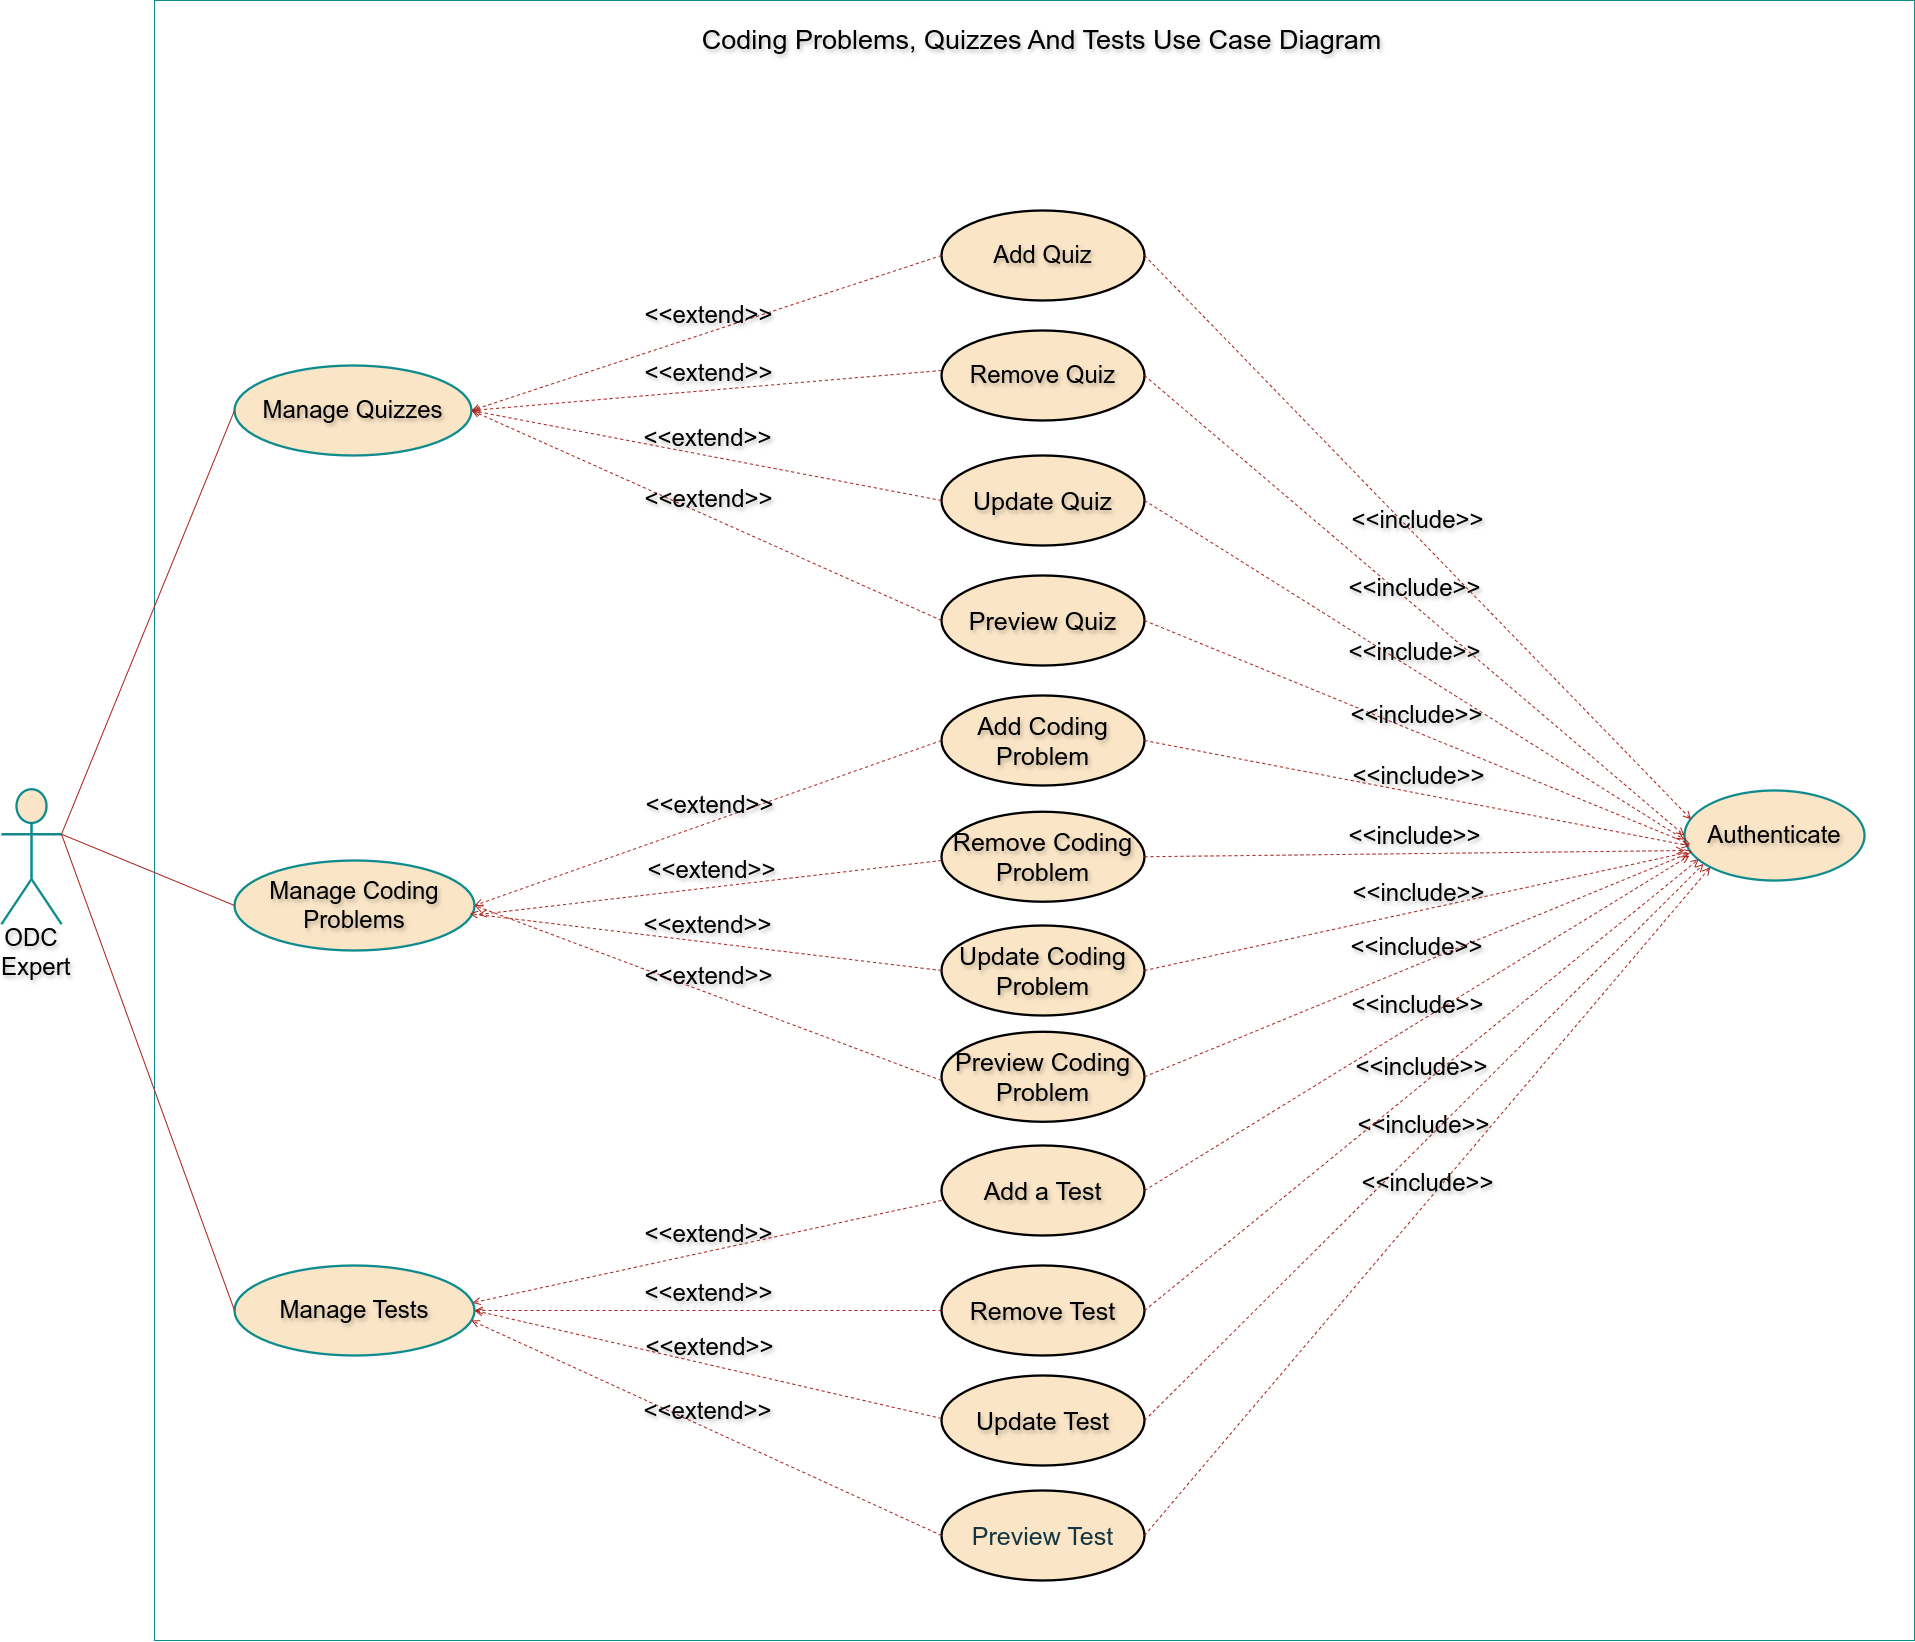
\includegraphics[width=1\textwidth, height=0.9\textheight]{images/usecaseSprint2.png}
  \caption{Sprint 3 Use Case Diagram}\label{fig: Sprint 3 Use Case Diagram}
\end{figure}

\newpage

\subsection{Use Case Description}
The following tables contain the description of the main use cases that we focussed on implementing during this sprint.

\subsubsection{Use Case Description for Creating a Quiz}

\normalsize
\begin{longtable}{|p{3cm}|p{12cm}|}
  \hline
  \rowcolor{green!20} \textbf{Use Case}    & \textbf{Create a Quiz}                                             \\ \hline
  \textbf{User Role}                       & \textbf{ODC Expert}                                                \\ \hline
  \textbf{Description}                     & The ODC Expert wants to create a new quiz.                         \\ \hline
  \textbf{Preconditions}                   & The ODC Expert is logged in to the system.                         \\ \hline
  \textbf{Postconditions}                  & A new quiz is created and added to the system.                     \\ \hline
  \multirow{10}{*}{\textbf{Main Scenario}} &
  1. ODC Expert selects the option to create a new quiz.                                                        \\ \cline{2-2}
                                           & 2. System prompts the ODC Expert to enter the name of the quiz.    \\ \cline{2-2}
                                           & 3. ODC Expert enters the name of the quiz.                         \\ \cline{2-2}
                                           & 5. ODC Expert adds tags to the quiz.                               \\ \cline{2-2}
                                           & 7. ODC Expert adds quiz questions.                                 \\ \cline{2-2}
                                           & 8. ODC Expert confirms to create the quiz.                         \\ \cline{2-2}
                                           & 9. System validates that the quiz has a name, tags, and questions. \\ \cline{2-2}
                                           & 10. System creates the quiz and adds it to the system.             \\ \hline
  \caption{Use Case Description for Creating a Quiz}\label{tab:create_quiz_use_case}
\end{longtable}

\subsubsection{Use Case Description for Adding a Problem}

\normalsize
\begin{longtable}{|p{3cm}|p{12cm}|}
  \hline
  \rowcolor{green!20} \textbf{Use Case}   & \textbf{Add Problem}                                                          \\ \hline
  \textbf{User Role}                      & \textbf{ODC Expert}                                                           \\ \hline
  \textbf{Description}                    & The ODC Expert wants to add a new problem to the system.                      \\ \hline
  \textbf{Preconditions}                  & The ODC Expert is logged in to the system.                                    \\ \hline
  \textbf{Postconditions}                 & A new problem is added to the system.                                         \\ \hline
  \multirow{7}{*}{\textbf{Main Scenario}} & 1. ODC Expert selects the option to add a new problem.                        \\ \cline{2-2}
                                          & 2. System prompts the ODC Expert to enter the name of the problem.            \\ \cline{2-2}
                                          & 3. ODC Expert enters the name of the problem.                                 \\ \cline{2-2}
                                          & 4. System prompts the ODC Expert to write the problem description.            \\ \cline{2-2}
                                          & 5. ODC Expert writes the problem description.                                 \\ \cline{2-2}
                                          & 6. System prompts the ODC Expert to add the problem function/class signature. \\ \cline{2-2}
                                          & 7. ODC Expert adds the problem function/class signature.                      \\ \cline{2-2}
                                          & 8. ODC Expert adds problem test cases.                                        \\ \cline{2-2}
                                          & 9. ODC Expert confirms to create the problem.                                 \\ \cline{2-2}
                                          & 10. System creates the problem and adds it to the system.                     \\ \hline
  \caption{Use Case Description for Adding a Problem}\label{tab:add_problem_use_case}
\end{longtable}

\subsubsection{Use Case Description for Creating a Test}

\normalsize
\begin{longtable}{|p{3cm}|p{12cm}|}
  \hline
  \rowcolor{green!20} \textbf{Use Case}   & \textbf{Create Test}                                                              \\ \hline
  \textbf{User Role}                      & \textbf{ODC Expert}                                                               \\ \hline
  \textbf{Description}                    & The ODC Expert wants to create a new test by selecting a quiz and a problem.      \\ \hline
  \textbf{Preconditions}                  & The ODC Expert is logged in to the system and has access to quizzes and problems. \\ \hline
  \textbf{Postconditions}                 & A new test is created and added to the system.                                    \\ \hline
  \multirow{6}{*}{\textbf{Main Scenario}} & 1. ODC Expert selects the option to create a new test.                            \\ \cline{2-2}
                                          & 2. ODC Expert enters the name of the test.                                        \\ \cline{2-2}
                                          & 3. ODC Expert searches for a quiz.                                                \\ \cline{2-2}
                                          & 4. ODC Expert selects a quiz.                                                     \\ \cline{2-2}
                                          & 5. ODC Expert searches for a problem.                                             \\ \cline{2-2}
                                          & 6. ODC Expert selects a problem.                                                  \\ \cline{2-2}
                                          & 7. ODC Expert confirms to create the test.                                        \\ \cline{2-2}
                                          & 8. System creates the test and adds it to the system.                             \\ \hline
  \caption{Use Case Description for Creating a Test}\label{tab:create_test_use_case}
\end{longtable}


\section{Analysis And Design}

\subsection{User Interface Design}
When designing the user interfaces we where committed to use Typescript to introduce type safety to our code.
and define the structure of the different objects in our application whether it is a quiz, a problem a test etc.
To achieve that, we used the rich Typescript type system to define the shape of our complex data structures.
as an example, the following code snippet represented in figure \ref{Code submit result type definition}
shows how we defined the structure of code submit result in our application.
we used techniques like union types, intersection types, and type aliases to have a level of certainty when writing
code, this helped us massively reduce the number of runtime errors and bugs.

\begin{figure}[h!]
  \centering
  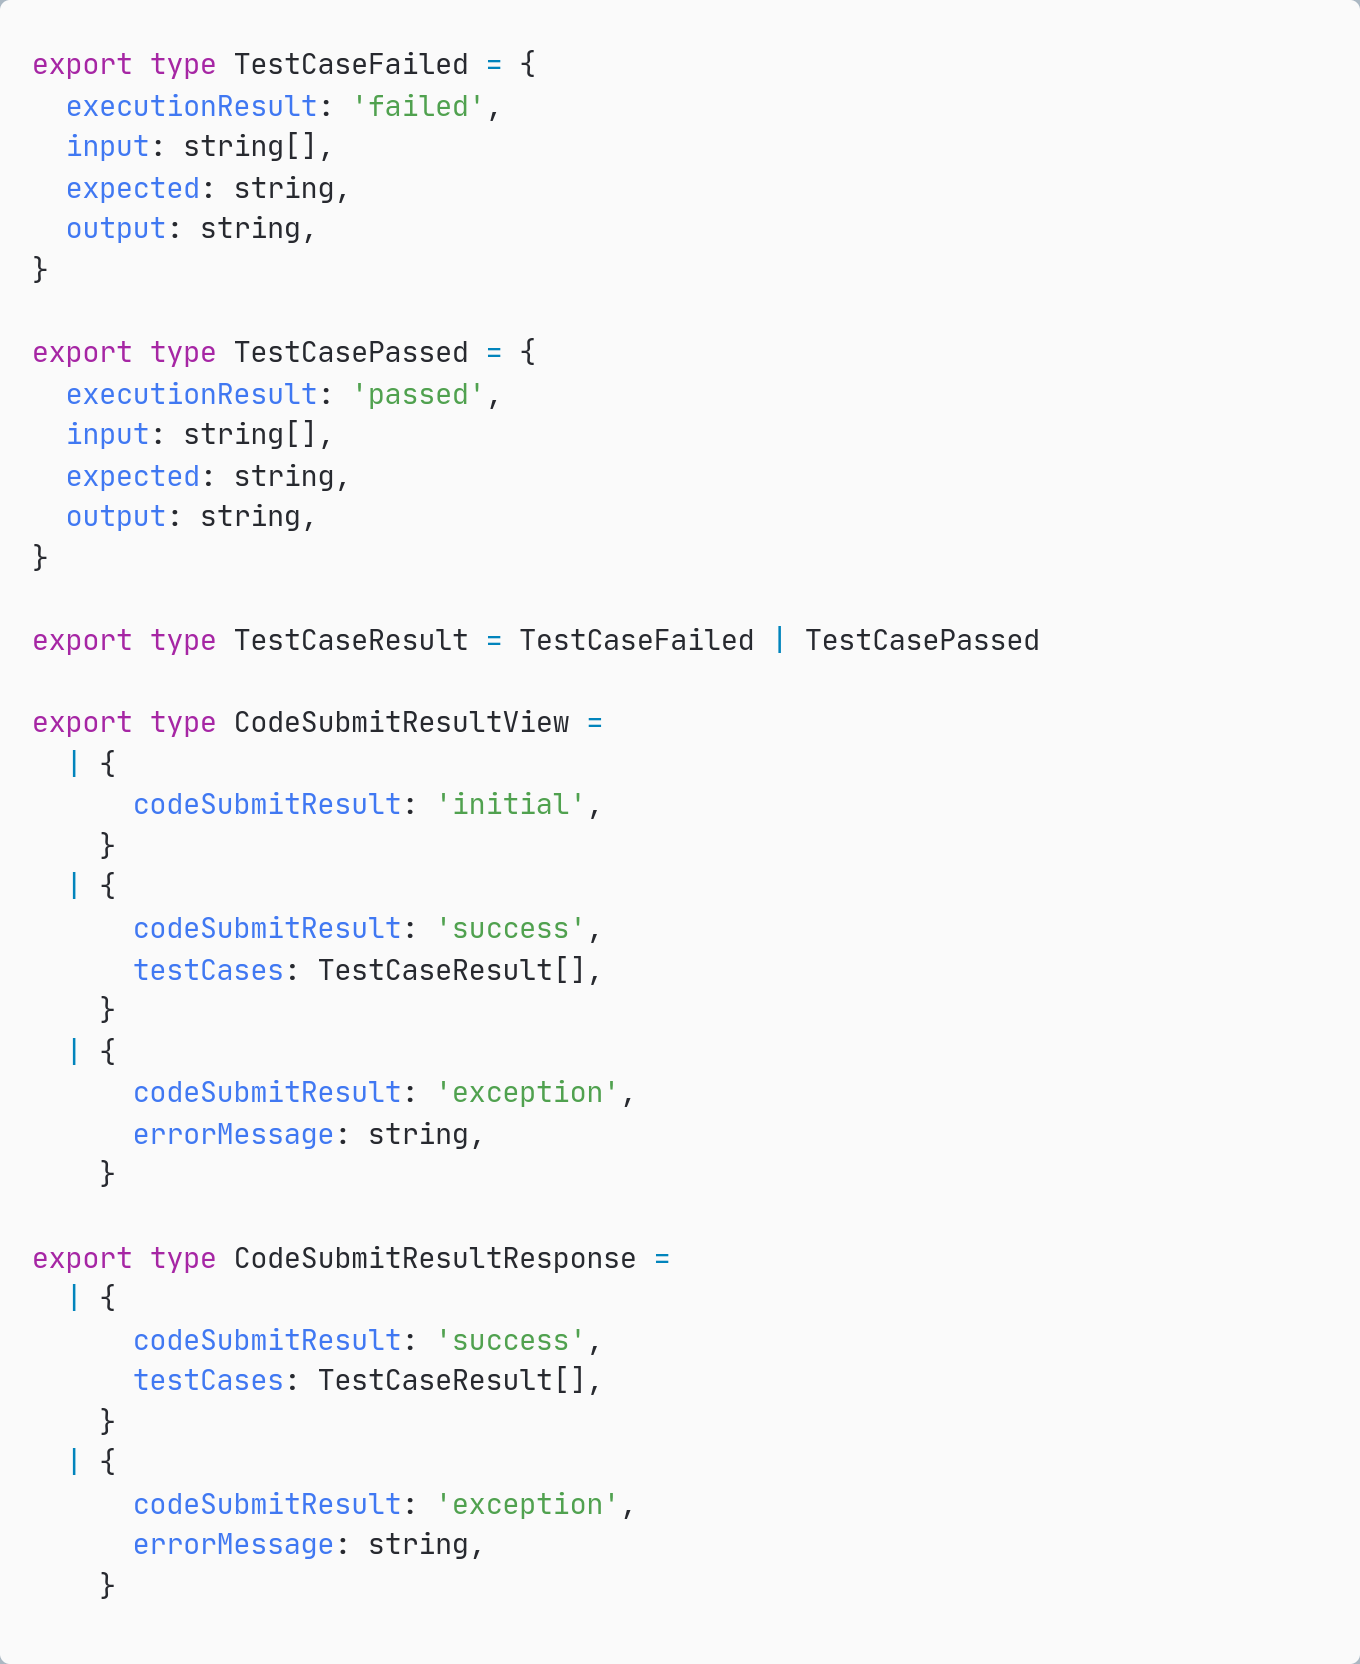
\includegraphics[width=1\textwidth]{images/types.png}
  \caption{Code submit result type definition}\label{Code submit result type definition}
\end{figure}

\newpage
\subsection{Building The Code Editor}
One of the main features that we needed to implement in this sprint is the code editor.
the code editor is a crucial part of our application as it is the main tool that the ODC Expert will use
to write the coding problems and test cases, and will be used by the candidates to solve the coding problems.
Implementing a code editor from scratch is a challenging task, but we were lucky to have a powerful library
called Monaco Editor that we used to build our code editor. Monaco Editor is the code editor that powers Visual Studio Code,
it is a powerful code editor that supports many features like syntax highlighting, code completion, and code linting.
It is also highly customizable and can be extended to support many languages and features. In general it was a great choice
to use it as a code editor in our application.

\begin{figure}[h]
  \centering
  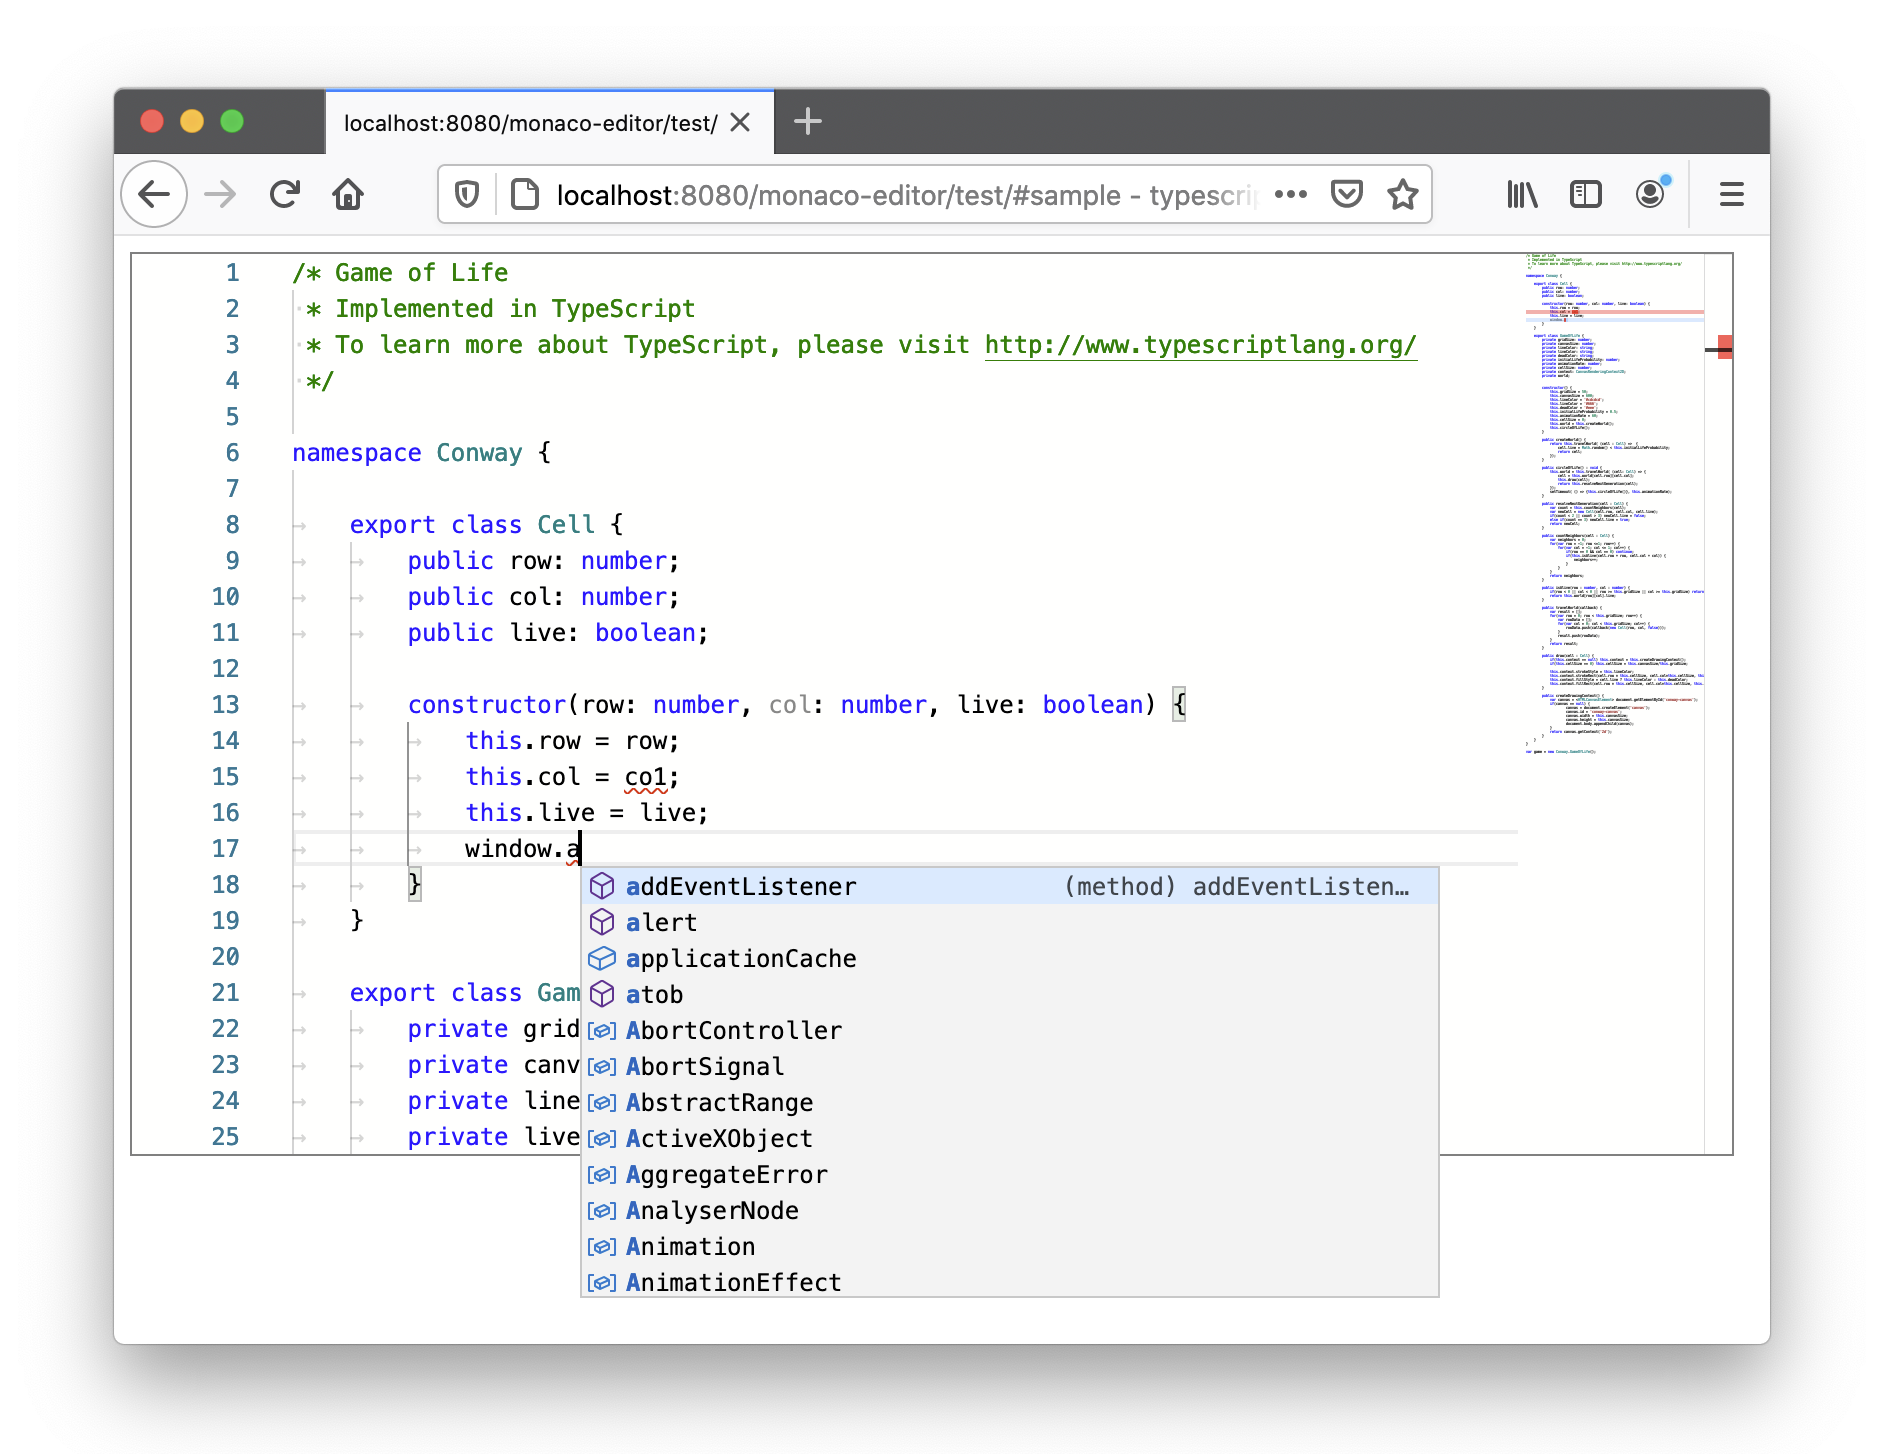
\includegraphics[width=1\textwidth]{images/monaco.png}
  \caption{Monaco Code Editor Preview}\label{Monaco Code Editor Preview}
\end{figure}

\subsection{Create Problem Sequence Diagram}
To Create a problem the ODC Expert will follow a sequence of steps described in the following sequence diagram.

\begin{figure}[h!]
  \centering
  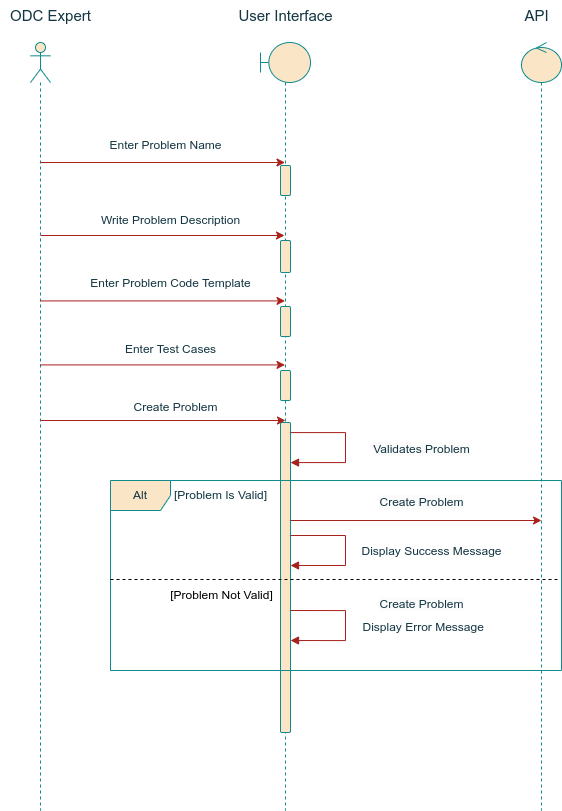
\includegraphics[width=0.8\textwidth, height=0.8\textheight]{images/seq_createProblem.png}
  \caption{Create Problem Sequence Diagram}\label{Create Problem Sequence Diagram}
\end{figure}

\subsection{Create Test Sequence Diagram}
Creating a test is a complex process that involves selecting a quiz and a problem, and then creating the test.
The following sequence diagram represents the steps that the ODC Expert will follow to create a test.

\begin{figure}[h]
  \centering
  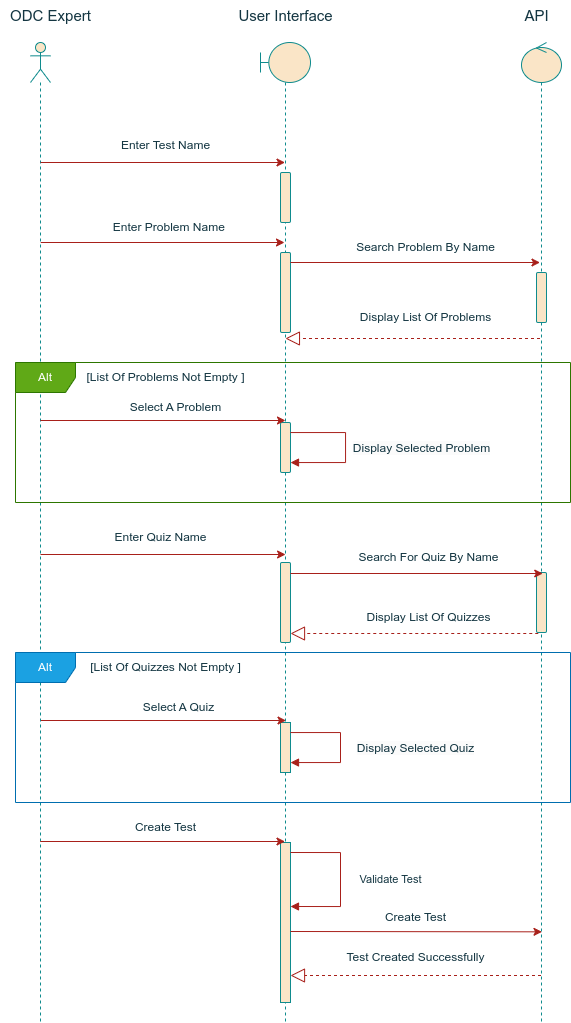
\includegraphics[width=0.9\textwidth, height=0.9\textheight]{images/seq_createTest.png}
  \caption{Create Test Sequence Diagram}\label{Create Test Sequence Diagram}
\end{figure}


\section{Implementation}
In this section we showcase the end results of the user interfaces that we have implemented in this sprint.

\subsection{Create Quiz Page}
The figure \ref{Create Quiz Page} shows the user interface for creating a quiz.
the ODC Expert can fill the form to create a new quiz and then save it to the system.

\begin{sidewaysfigure}
  \centering
  \setlength\fboxsep{0pt} % Adjusts the separation between the image and the border
  \setlength\fboxrule{2pt} % Adjusts the thickness of the border
  \fcolorbox{orange}{white}{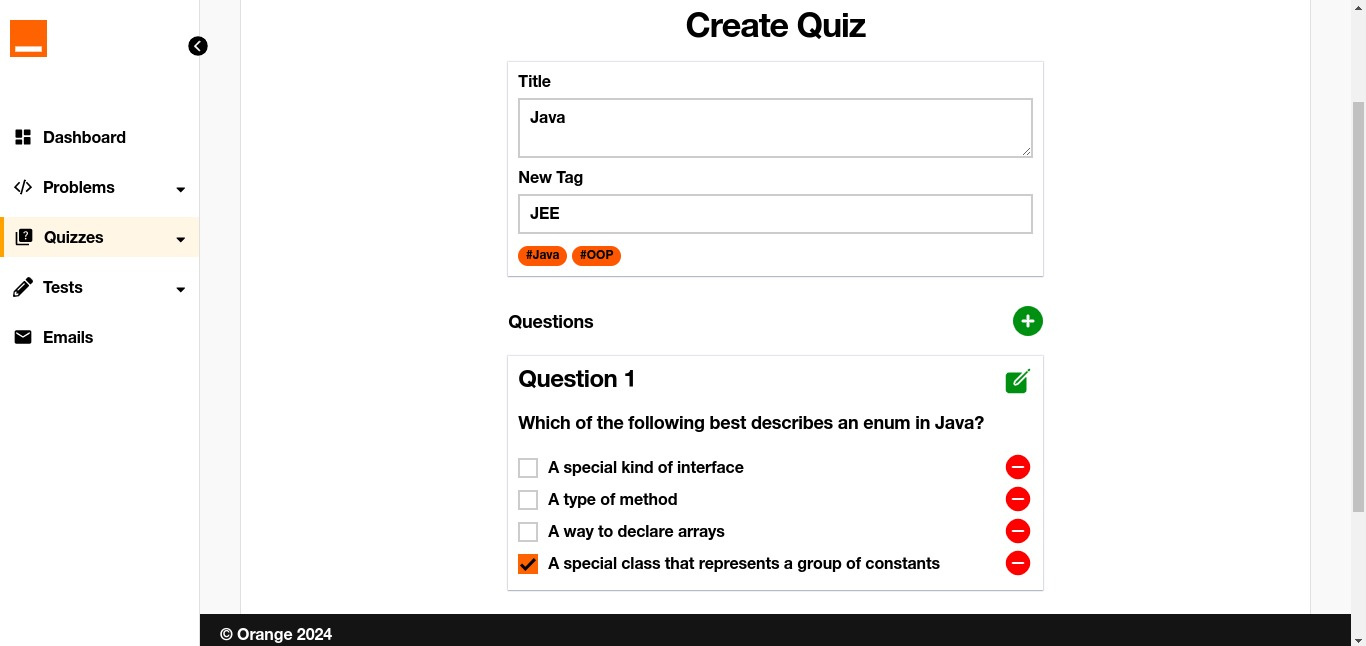
\includegraphics[width=0.8\paperheight, height=0.6\paperwidth]{images/createQuiz.jpeg}}
  \caption{Create Quiz Page}\label{Create Quiz Page}
\end{sidewaysfigure}

\subsection{Create Problem Page}
The figure \ref{Create Problem Page} shows the user interface for creating a problem.
the ODC Expert can fill the form to create a new problem and then save it to the system.

\begin{sidewaysfigure}[h!]
  \centering
  \setlength\fboxsep{0pt} % Adjusts the separation between the image and the border
  \setlength\fboxrule{2pt} % Adjusts the thickness of the border
  \fcolorbox{orange}{white}{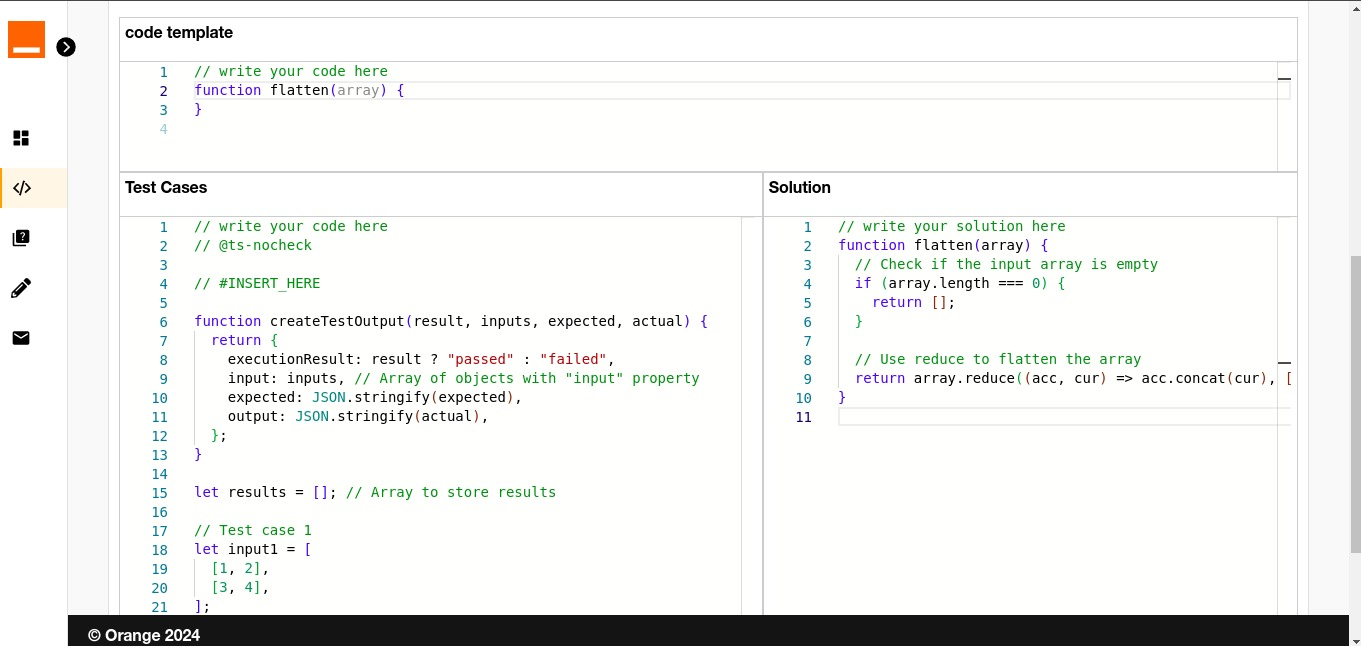
\includegraphics[width=0.8\paperheight, height=0.6\paperwidth]{images/createProblem.jpeg}}
  \caption{Create Problem Page}\label{Create Problem Page}
\end{sidewaysfigure}

\subsection{Create Test Page}
The figure \ref{Create Test Page} shows the user interface for create a test.
the ODC Expert can fill the form to create a new test and then save it to the system.

\begin{sidewaysfigure}[h!]
  \centering
  \setlength\fboxsep{0pt} % Adjusts the separation between the image and the border
  \setlength\fboxrule{2pt} % Adjusts the thickness of the border
  \fcolorbox{orange}{white}{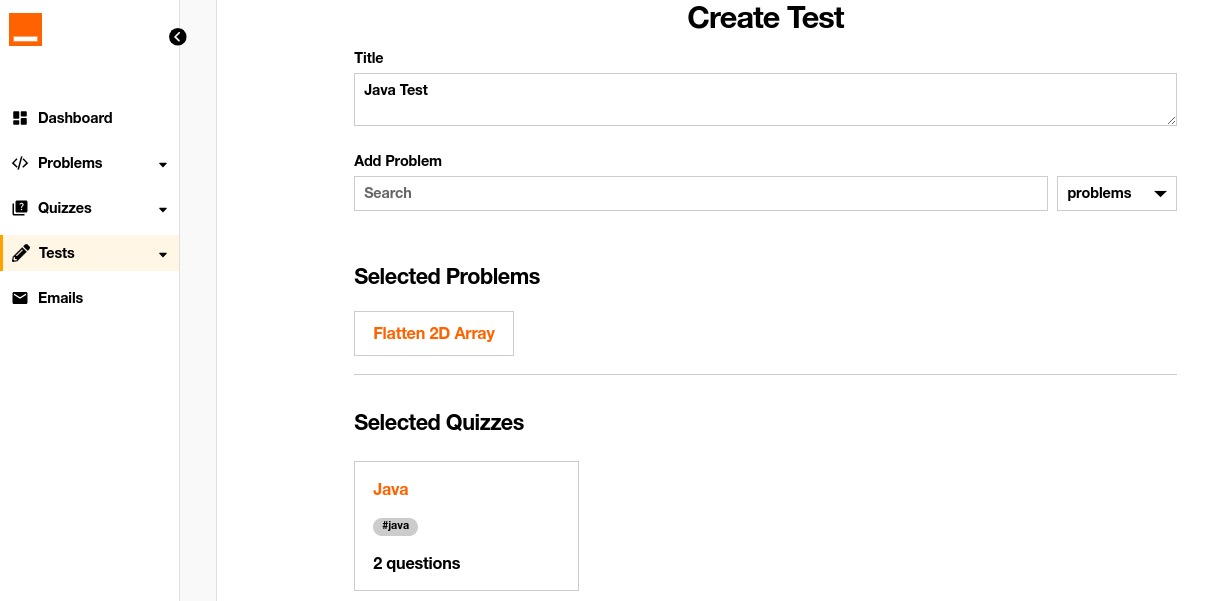
\includegraphics[width=0.8\paperheight, height=0.6\paperwidth]{images/creatTest.jpeg}}
  \caption{Create Test Page}\label{Create Test Page}
\end{sidewaysfigure}

\subsection{Preview Problem Page}
the figure \ref{Preview Problem Page} shows the user interface for previewing a problem.

\begin{sidewaysfigure}[h!]
  \centering
  \setlength\fboxsep{0pt} % Adjusts the separation between the image and the border
  \setlength\fboxrule{2pt} % Adjusts the thickness of the border
  \fcolorbox{orange}{white}{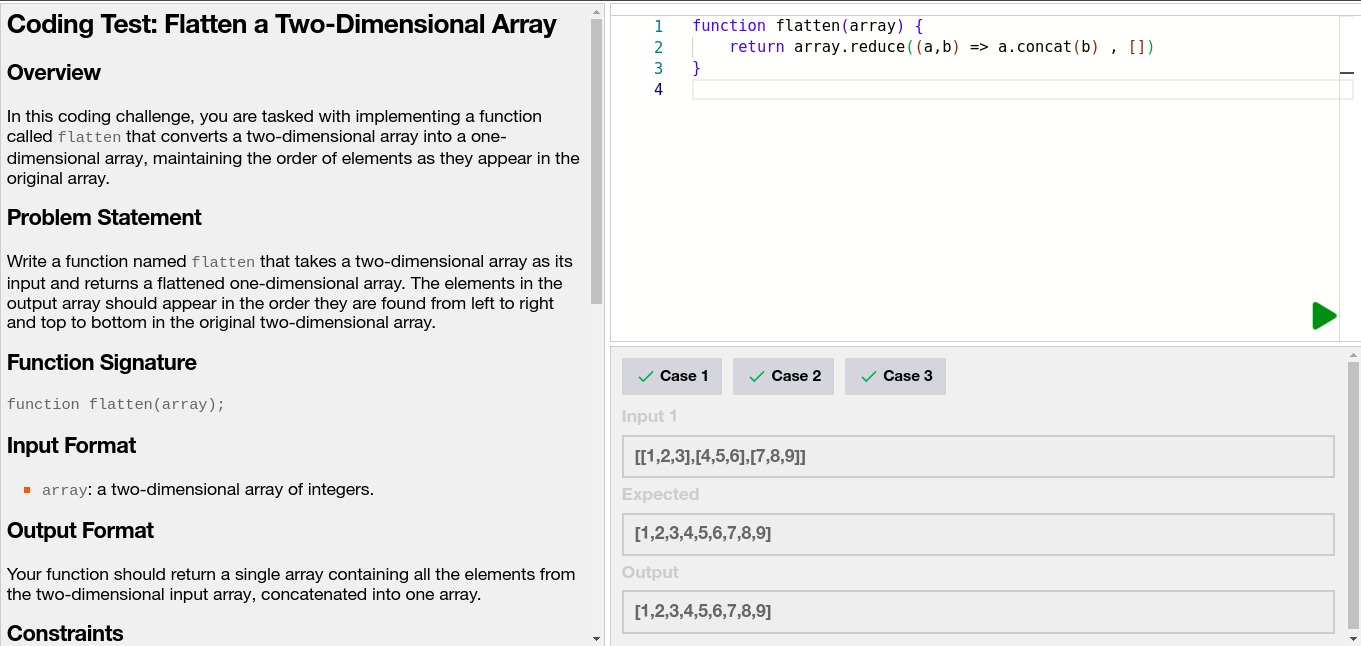
\includegraphics[width=0.8\paperheight, height=0.6\paperwidth]{images/previewProblem.jpeg}}
  \caption{Preview Problem Page}\label{Preview Problem Page}
\end{sidewaysfigure}

